\chapter{Schnittstellen \& Protokolle}
	\begin{description}
		\item[Channel] Beschreibt die Channelschnittstelle. Implementatoren eines eigenen Channels müssen sich an diese Schnittstelle halten sowie den Channel in der appConfiguration eintragen.
		\item[Contactbook] Beschreibt die Contactbookschnittstelle. Implementatoren eines eigenen Contactbooks müssen sich an diese Schnittstelle halten sowie das Contactbook in der appConfiguration eintragen.
		\item[datachannelMessage] Beschreibt den Aufbau der Messages, die über den Data-Channel der PeerConnection gesendet werden.
		\item[signalingChannel] Beschreibt den Aufbau der Messages, die über den Signaling-Channel gesendet werden.
	\end{description}

	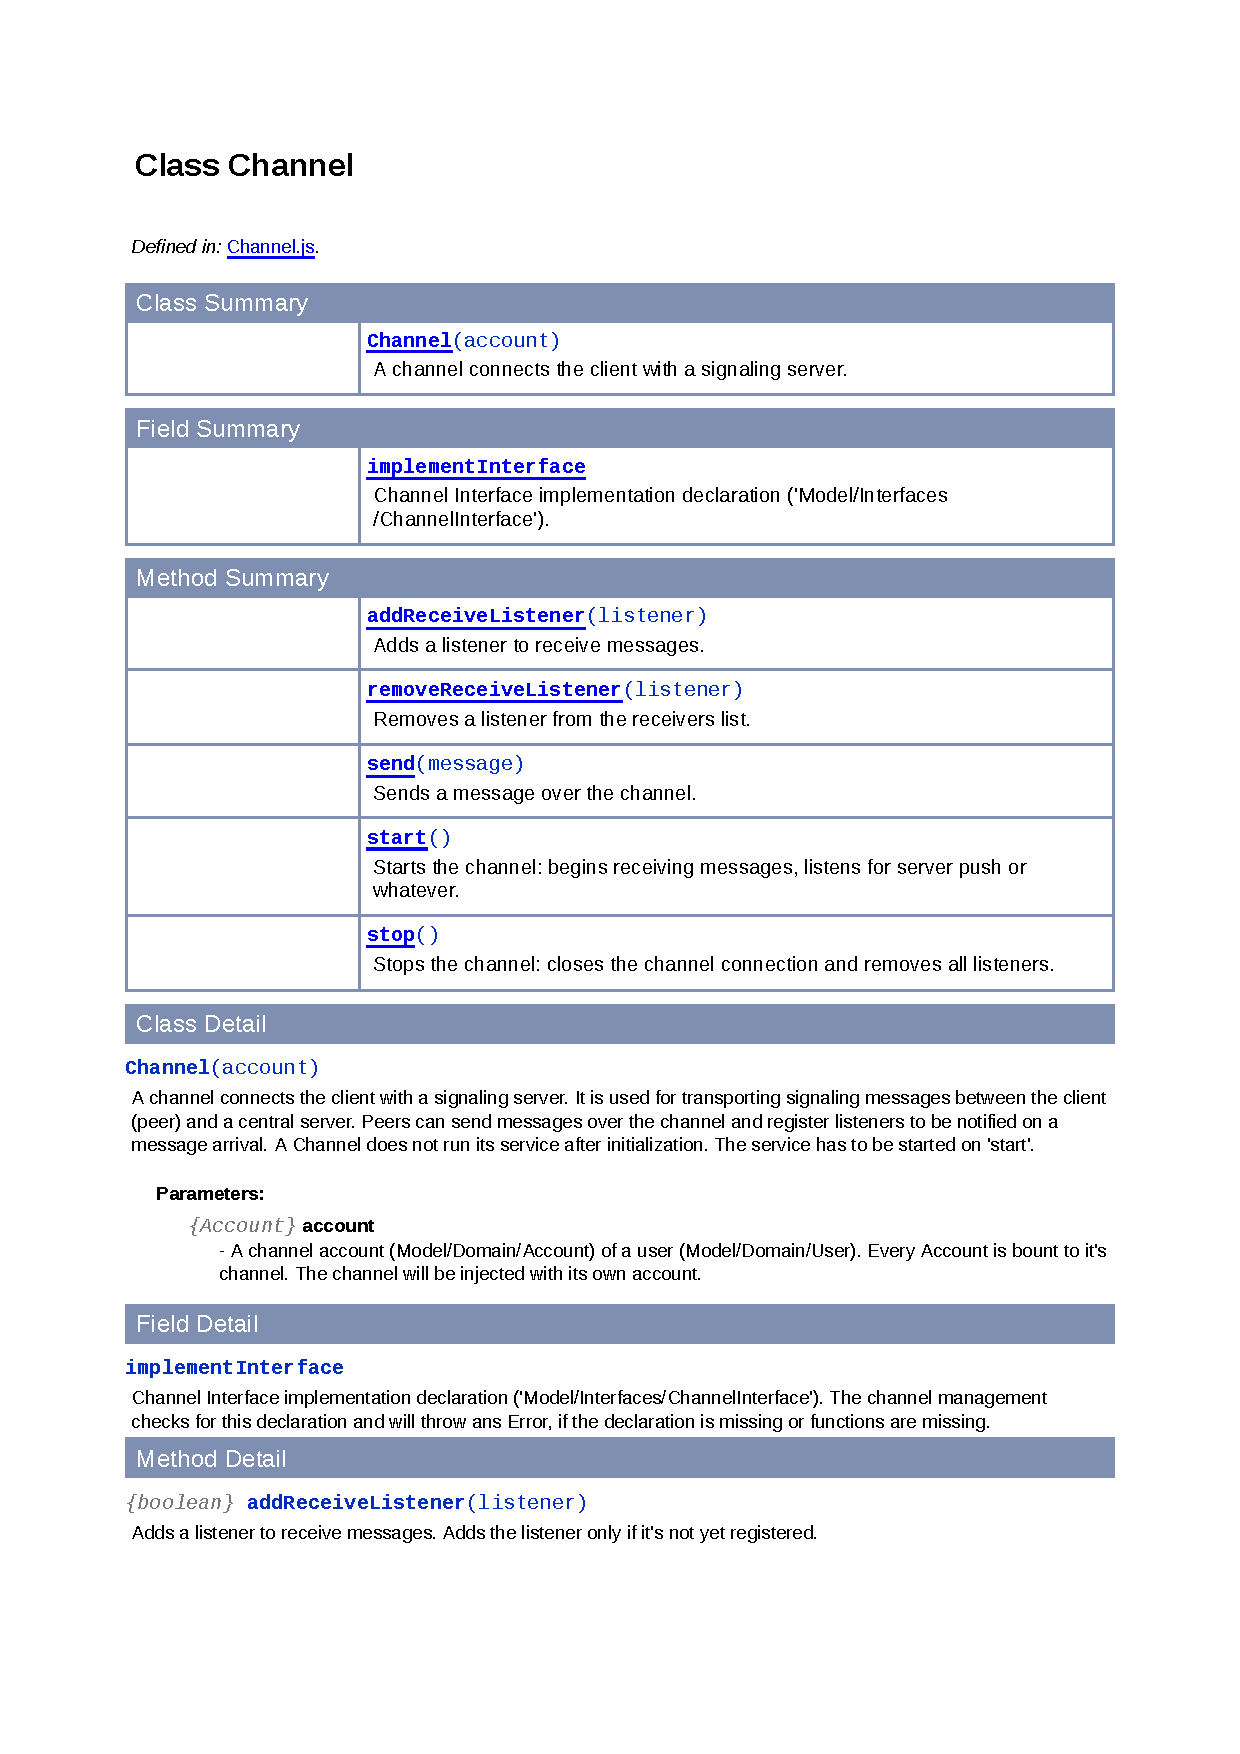
\includepdf[pages=-]{../interfacesAndProtocols/Channel.pdf}
	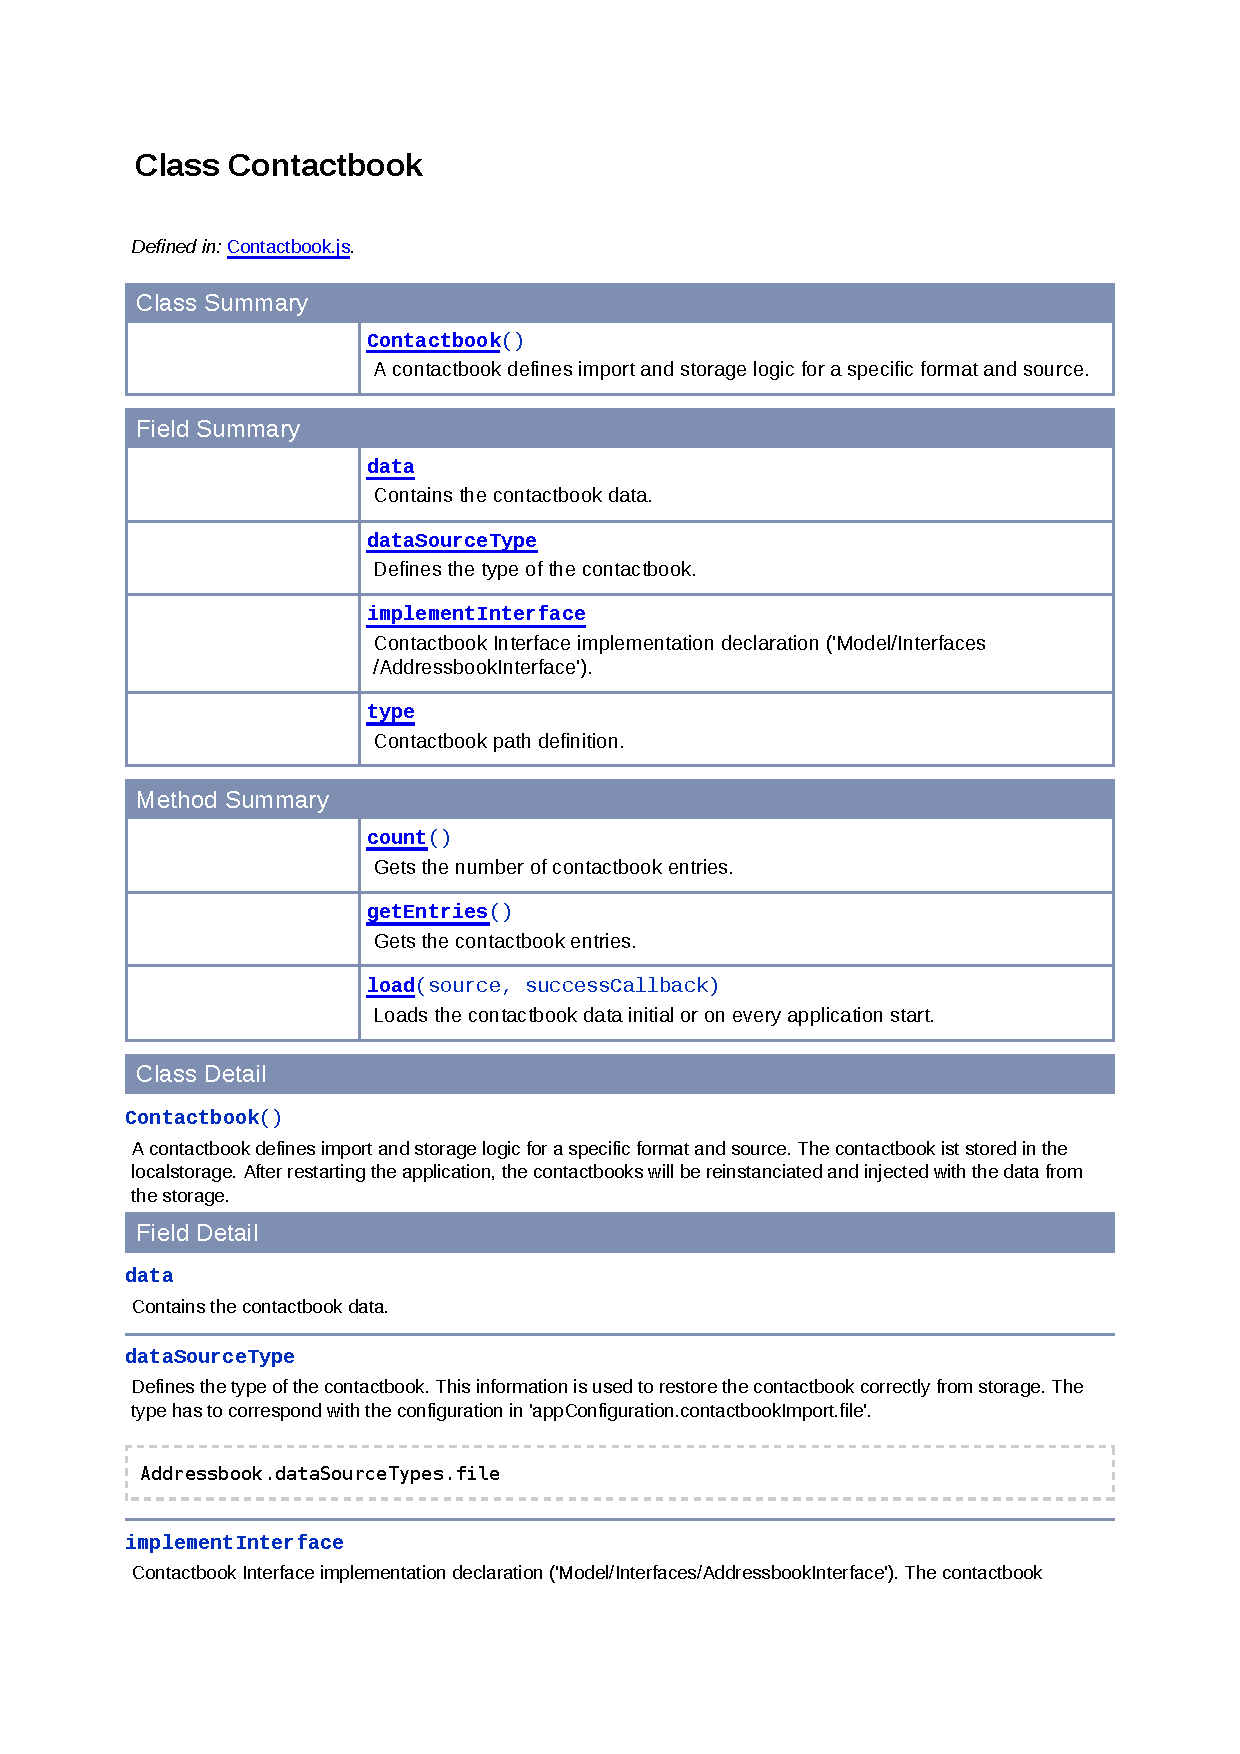
\includepdf[pages=-]{../interfacesAndProtocols/Contactbook.pdf}
	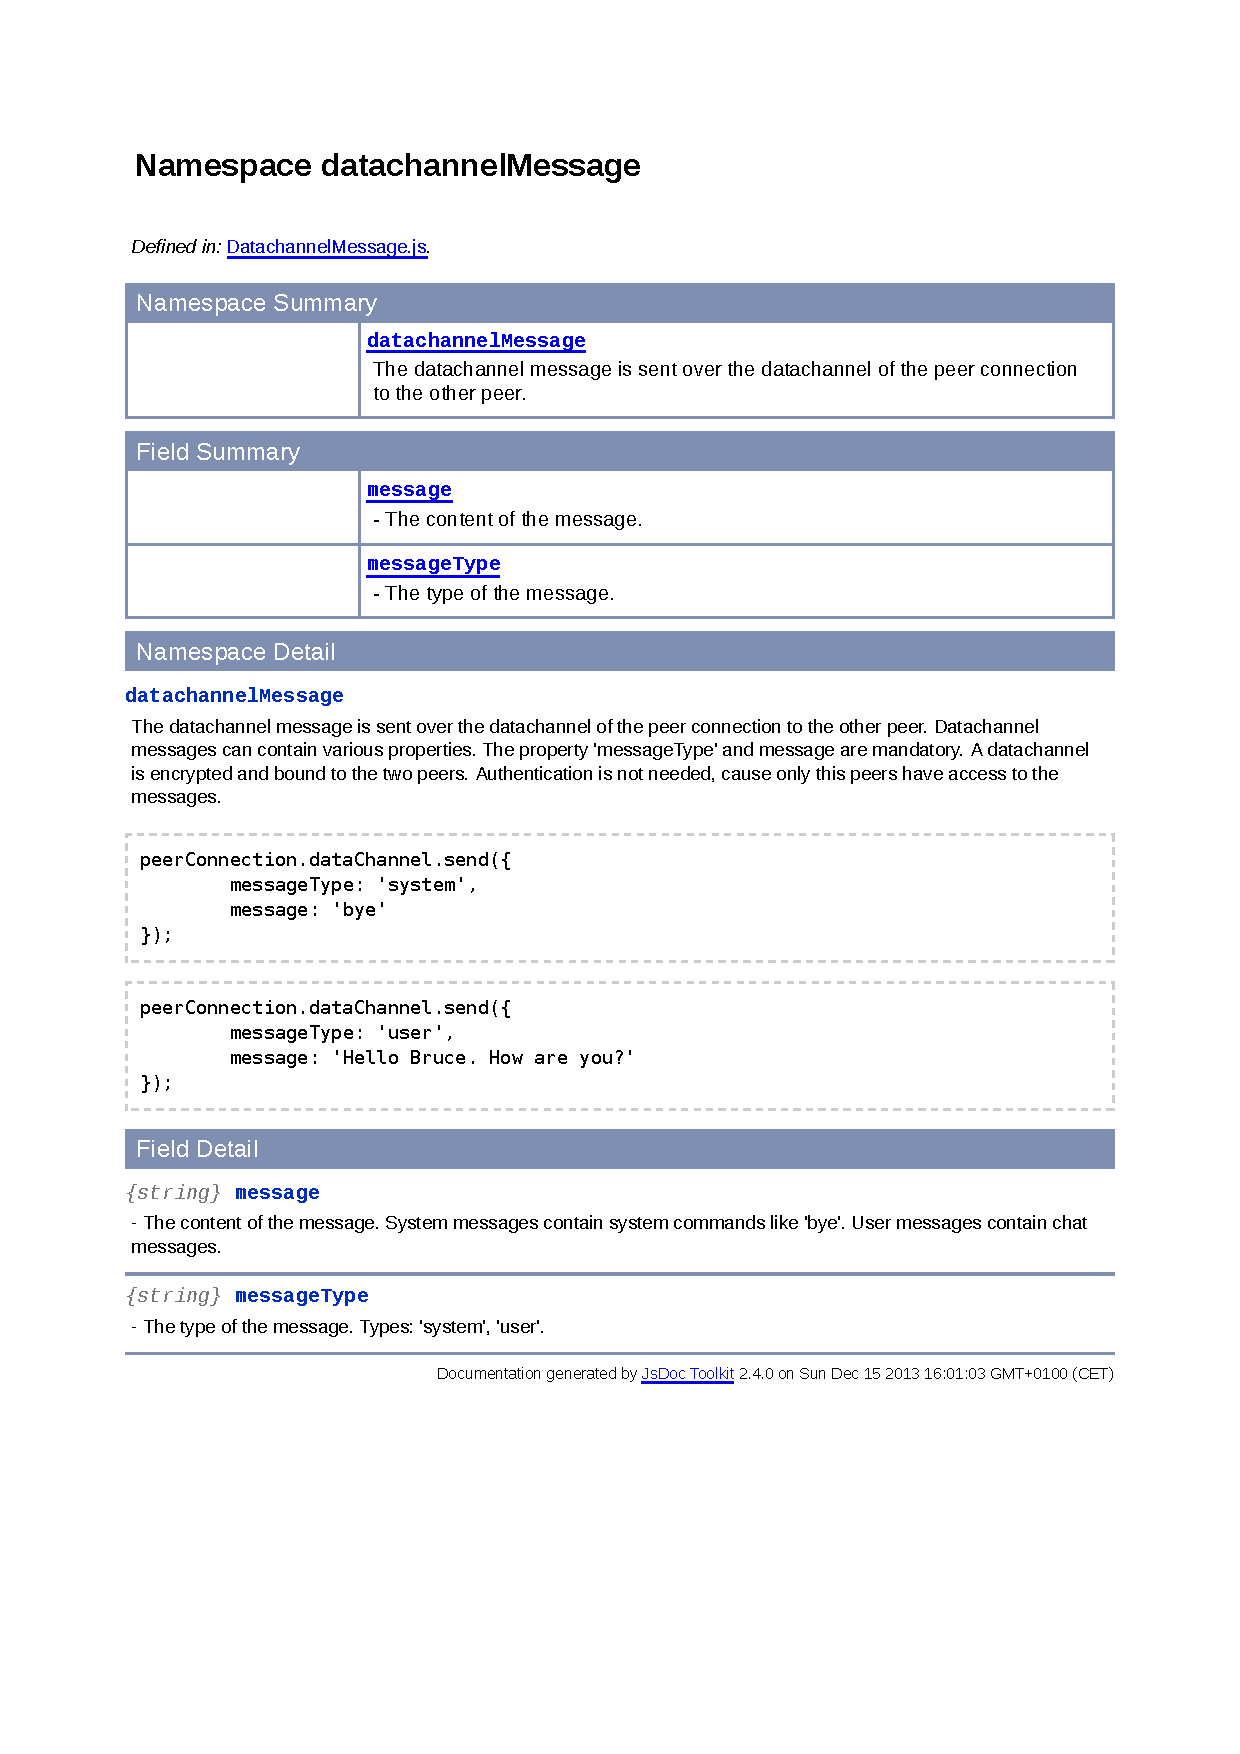
\includepdf[pages=-]{../interfacesAndProtocols/datachannelMessage.pdf}
	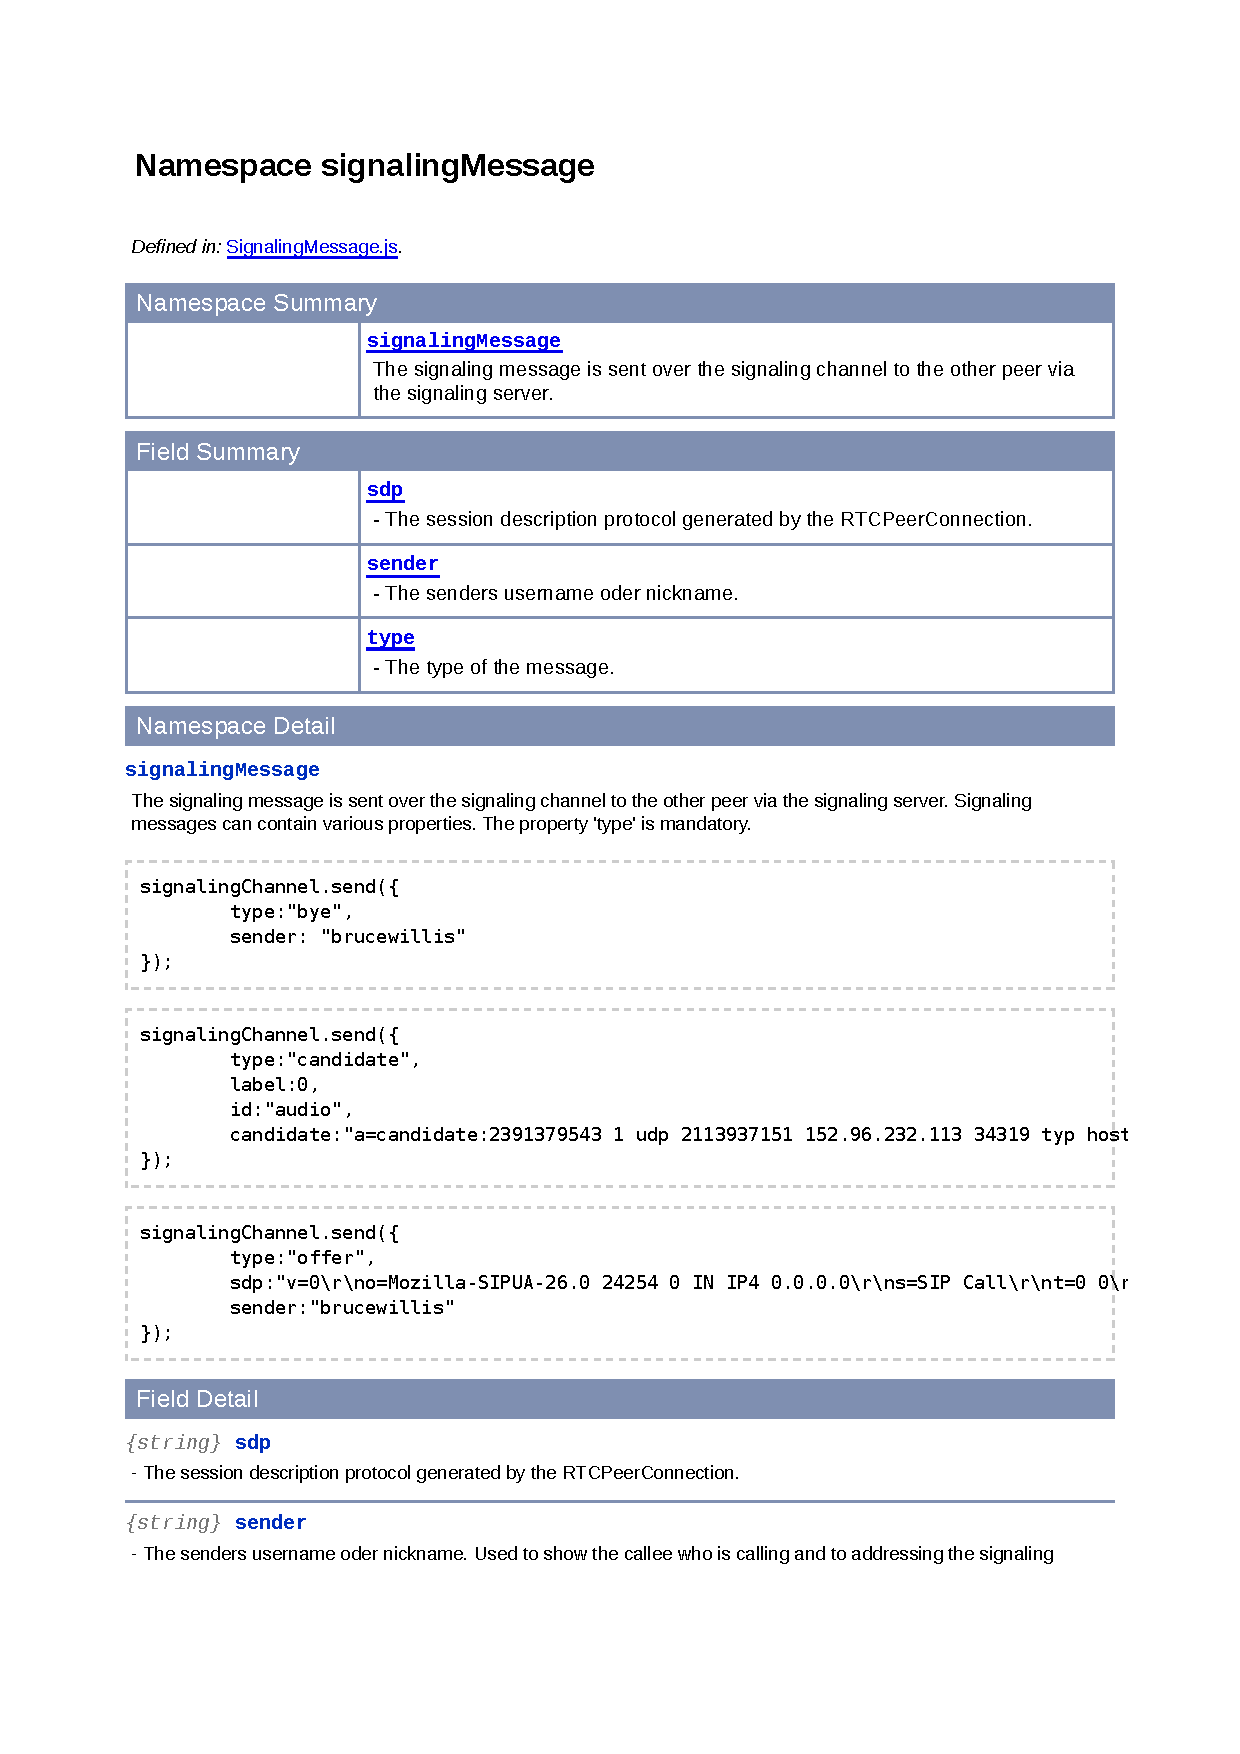
\includepdf[pages=-]{../interfacesAndProtocols/signalingMessage.pdf}